% Results. Numbers: results_em/ (see README.md of the repository).
\section{Results}
\label{sec:results}

\subsection{The reference colony follows Calhoun's sequence}
\label{sec:res-trajectory}

The time course of \Cone\ has the four phases of Universe~25 in Calhoun's order (Fig.~\ref{fig:trajectory}). On a
time axis relative to the peak of each system ($t_{\rm pk}$: the start of the plateau in the model, median week 34;
day 560 in Universe~25), births start at $0.09\,t_{\rm pk}$ and growth slows at $0.31\,t_{\rm pk}$ (Universe~25: 0.19
and 0.56). The mean competence of the adults falls below 0.5 at week 13, while the colony is still growing. Births
stop near the peak: 99\% of them have occurred by week 40 and the last one comes at week 59 [46, 76] (median and
10--90\% range over 200 runs). The shapes differ after the peak. The model stays on a plateau for about
$1.5\,t_{\rm pk}$ and then falls along a sigmoid as the closed cohort ages, whereas Universe~25 declined from its
peak; the model dies out at $4.97\,t_{\rm pk}$, week 169 (Kaplan--Meier median; 95\% interval [167, 171]; 10--90\%
range [157, 186]), against a projected $3.18\,t_{\rm pk}$ for Universe~25. The peak uses $0.36$ of the
damage-threshold capacity $\Kg=m_c|G|$ and leaves 16\% of the cells empty (Universe~25: about 20\% of the nest boxes
empty, an agreement in sign, since $|G|$ and $m_c$ were not calibrated). The model starts from 400 young adults
rather than four pairs, so the comparison is of shape, not of timing (doubling times: SM,
Section~\ref{SM-supp:patterns}).

\begin{figure}[!tp]
  \centering
  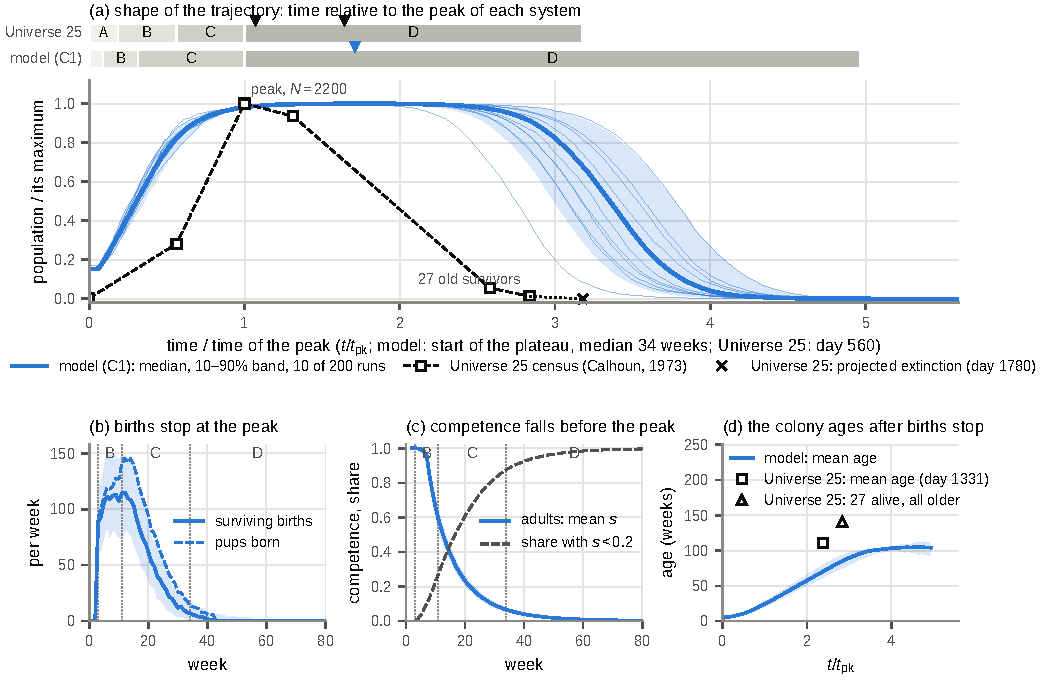
\includegraphics[width=0.9\textwidth]{fig_em_trajectory.pdf}
  \caption{The reference colony and Universe~25. (a)~Population relative to its maximum against time relative to
  the peak of each system, $t/t_{\rm pk}$ ($t_{\rm pk}$: start of the plateau, $N\ge0.98\max N$, in each run of the
  model, median week 34; day 560 in Universe~25). Model: \Cone, median, 10--90\% band and 10 of 200 colonies,
  rescaled run by run. Squares: census of Universe~25 \citep{Calhoun1973}; cross: Calhoun's projected extinction
  (day $1\,780$). Ribbons: phases A--D (A, adjustment; B, growth; C, slower growth; D, death phase) as dated by
  Calhoun and, for the model, as measured in each run (medians): first births, halving of the growth rate of $\ln N$,
  start of the plateau and extinction. Triangles: last surviving young and last conception in Universe~25, last birth
  in the model. No curve is fitted. (b)~Pups born and pups surviving birth per week. (c)~Mean reproductive
  competence of the adults and share of all animals with $s<0.2$. (d)~Mean age of the living animals against
  $t/t_{\rm pk}$; symbols: mean age of the survivors of Universe~25 on day $1\,331$, and the 27 survivors on day
  $1\,588$, all older than 987 days. Bands: 10--90\% of colonies. Dotted lines in (b, c): phase boundaries.}
  \label{fig:trajectory}
\end{figure}

\subsection{Adult recovery decides the outcome}
\label{sec:res-recovery}

Whether adults made non-breeding by crowding recover decides between collapse and persistence
(Fig.~\ref{fig:recovery}). If adults regain competence at a fraction $\eadult$ of the juvenile rate, every colony
still dies out for $\eadult\le0.02$ ($2\,880$ of $2\,880$ colonies at $L=15$ and 30, in space and well mixed, for
every $\lambda$; SM, Table~\ref{SM-tab:sm-pext}), so the collapse is not an artefact of the edge $\eadult=0$. Above a
threshold $\eadult^c$ the colony persists. In space the threshold falls with the side of the arena without visible
saturation: from 0.133 [0.113, 0.157] to 0.085 [0.073, 0.099] and 0.050 [0.037, 0.063] between $L=15$, 30 and 60
when recovery is individual ($\lambda=0$), and from 0.97 [0.88, $>$1] to 0.73 [0.67, 0.81] and 0.53 [0.46, 0.62]
when it is purely social ($\lambda=1$; profile-likelihood intervals of the midpoint; SM, Table~\ref{SM-tab:sm-epsc}).
Three sizes do not determine its limit for $L\to\infty$, which could be zero. Well mixed with global mating it also
falls (0.81, 0.51, 0.30, again with non-overlapping intervals); with mating in the cell it is resolved only to the
grid of $\eadult$ (0.80, 0.6--0.8, 0.60; overlapping intervals), compatible with the deterministic limit, 0.585.
With $\lambda\ge0.9$ no recovery rescues the well-mixed colony (all but one of $4\,860$ colonies die out), because
an adult whose recovery is social finds no competent demonstrators. The robust statement is therefore the edge: the collapse requires that adults recover
asocially at most slowly, $\eadult(1-\lambda)\approx0$, at the scale of the experiment.

The reversible-suppression null, \Cone\ with $\eadult=0.8$ and $\lambda=0.9$ (asocial recovery at 0.08 of the
juvenile rate), persists in all 200 colonies to week
$1\,000$. It keeps every spatial and deterioration pattern of \Cone\ (200 of 200 runs each; Fig.~\ref{fig:patterns},
first 600 weeks), and its natality nearly ceases after the peak (to 0.1\% of its maximum, median), so the two
outcomes share the first half of the sequence; but breeding then resumes. The collapse envelope separates them: the
end of natality, the absence of recovery and the extinction fail in all 200 runs. Nor does the colony settle. After
a plateau from week 34 to about week 100 (median) it falls to 0.15 of the peak (week 141) and then cycles with a
period of 148 [147, 149] weeks (peak to peak; mean over runs, 143--152 across runs, 10--90\%). The oscillations are
persistent and slowly damped. The peak-to-trough amplitude decays from 0.85 of the first peak to 0.49, 0.42 and 0.39
in the next three cycles and then only slowly ($-0.013$ [$-0.017$, $-0.008$] of the first peak per 100 weeks over
cycles 3--5, about 3\% of the amplitude), so that at week $1\,000$ the colony still oscillates between about 0.40
and 0.80 of the first peak. Whether the amplitude levels off (a geometric fit gives 0.35 [0.33, 0.37]) or keeps
decaying cannot be decided within $1\,000$ weeks. The autocorrelation of $N$ over weeks 300--1000, corrected for the
shrinking overlap of the lagged series, is 0.90 at one, two and three periods (0.71, 0.51 and 0.34 uncorrected),
which rules out a fast-relaxing quasi-cycle. In all 200 runs the evaluation
thus finds cycles with recovery of births and no logistic saturation: the trajectory differs in form, not only in
level. With initial ages spread over 4--80 weeks the null falls to 0.23 [0.21, 0.25] of the peak and cycles with the
same period, so the cycle is not an artefact of the synchronous founding cohort.

Earlier confined colonies, not used to build or tune the model, allow only a consistency check of this branch,
since its persistence follows from the choice of $\eadult$ above the threshold. With food in excess those colonies
stopped growing below the limit set by food, mainly through the failure of litters to survive
\citep{Southwick1955a,Southwick1955}; confined populations of several rodent species regulated their density
\citep{Lidicker1965}; and confined deermice of asymptotic populations did not breed until removed from them
\citep{Terman1973}. Scored on the null (re-run with the archived seeds to record every litter), litter loss is
concentrated on the plateau: the fraction of litters with no surviving pup rises from 0.05 during growth to 0.24
[0.24, 0.25] (0.09 in \Cone) and falls back to 0.07--0.10 afterwards. But the fall of natality is mainly a fall of
conception (73\% of its logarithmic decline), so this pattern is reproduced only in part. Most females born on the
plateau never breed (0.89 do not conceive by 48 weeks of age), but so do those of \Cone\ (0.96). In \Cone\ no female
is born after the plateau, whereas in the null those born during the decline breed (only 0.37 do not conceive by 48
weeks; 0.72 of those born from week 300 on); what separates the outcomes is whether adults resume breeding
(definitions and sources of these held-out patterns: SM, Section~\ref{SM-supp:recovery}). The quick recovery of deermice removed from the asymptotic population
is reproduced by construction: phase-D animals of \Cone\ moved to an enclosure where adults recover
individually found a colony in 51 of 60 trials (Fig.~\ref{fig:behaviour}e), whereas Calhoun's transplants bred very
poorly \citep{Marsden1972}, the pattern of the irreversible branch.

\begin{figure}[!tp]
  \centering
  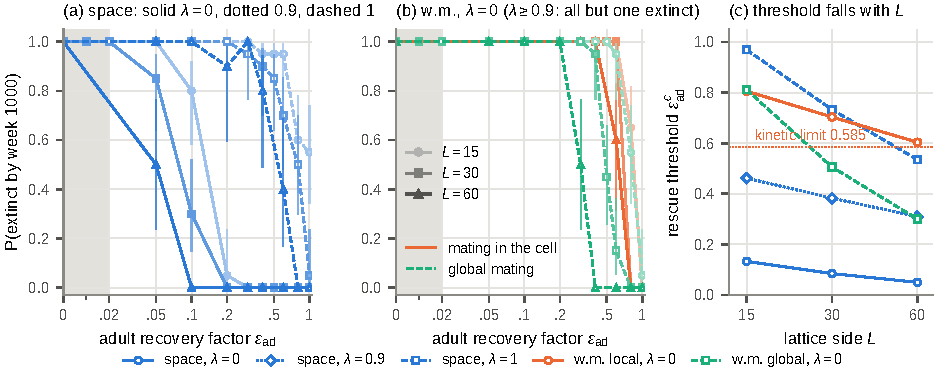
\includegraphics[width=\textwidth]{fig_em_recovery.pdf}
  \caption{Adult recovery decides the outcome. Probability that a \Cone\ colony is extinct by week $1\,000$ against
  the adult recovery factor $\eadult$ (fraction of the juvenile rate). (a)~Spatial model (with retreat sites),
  individual ($\lambda=0$, solid), mostly social ($\lambda=0.9$, dotted) or purely social recovery ($\lambda=1$,
  dashed). (b)~Well-mixed model, $\lambda=0$, mating in the cell (orange) or global (green); with $\lambda\ge0.9$ all
  but one of the $4\,860$ well-mixed colonies (three mating rules) die out. Shades and markers: $L=15$, 30, 60 (20, 20 and 10 colonies per point; 95\% Wilson intervals
  where $0<P<1$). Grey band: every colony collapses. (c)~Rescue threshold $\eadult^c$ (midpoint of a logistic fit)
  against $L$; dotted: value of the kinetic equation, 0.585. Data: SM, Tables~\ref{SM-tab:sm-pext}
  and~\ref{SM-tab:sm-epsc}.}
  \label{fig:recovery}
\end{figure}

\subsection{The collapse needs neither space nor the four social rules}
\label{sec:res-wm}

Removing space requires a control (Fig.~\ref{fig:wellmixed}e). When every animal is relocated at random each week
but mates only within its cell, the deformation is extinctive in itself: the short-lived control, which in space is
still alive in 89 of 200 colonies at week $1\,000$, dies out in 200 of 200 well-mixed colonies (median 120 weeks,
earlier than \Cone, 147), through a mate-finding Allee effect after the overshoot. The test therefore rests on
global mating, in which a female mates with a reproductive male drawn from the whole arena. There the control lives
far longer than \Cone\ and persists in larger arenas (extinct by week $1\,000$: 81, 1 and 0 of 200 at $L=30$, 45
and 60; at $L=30$ all colonies die out by week $3\,000$), whereas \Cone\ dies out in all 600 colonies at 138--140
weeks, almost independently of $L$. The core model without the four social rules collapses as well, in space and in
both well-mixed variants (all $1\,000$ colonies; median extinction at 136--166 weeks). The core model and the
short-lived control share the same slow individual recovery at every age ($r=0.01$); well mixed, where attraction
($\alpha$, 4 in the core and 1.4 in the control) plays no role, only the long life span of the core makes it
collapse. The cessation of breeding and the extinction thus need neither space nor the four social
rules: they need crowding damage and long-lived adults that recover slowly, if at all
(Section~\ref{sec:res-recovery}). A component
Allee effect remains with global mating, because a female paired with an incompetent male conceives with
probability $p_0s_fs_m$.

Without space the end of natality and the extinction are the same, but the sequence is not. With mating in the
cell, growth stays fast and competent until the peak (a socially functional growth phase in 200 of 200 runs, against
4 of 200, and 194 marginal, in space), the peak is 2.3 times denser (6.6 against 2.9 animals per cell), and
competence then collapses at once, so that phase~C lasts two weeks (weeks 24--26), against 23 weeks in space and
about 35 in Universe~25. With global mating phase~C lasts 11 weeks (weeks 7--18), so the compression comes from local
mating, not from the absence of space. Space also changes how the colony is organised. At the spatial
peak the mean occupancy is 2.9 animals per cell, but it is aggregated (variance-to-mean ratio 2.53 [2.51, 2.55];
maximum about 16) and 18\% [18, 19] of the animals sit in cells above $m_c$ (SM, Figs.~\ref{SM-fig:occupancy}
and~\ref{SM-fig:snapshots}): the colony crowds into pools next to empty cells and lodges a class of withdrawn
non-breeders, isolated adults with $s<0.2$ that appear already during growth and sit mostly in the retreat
sites; well mixed the occupancy is homogeneous and almost nobody stays isolated. That class cannot form under random
relocation, so its absence there is a consistency check, not a finding.

\begin{figure}[!tp]
  \centering
  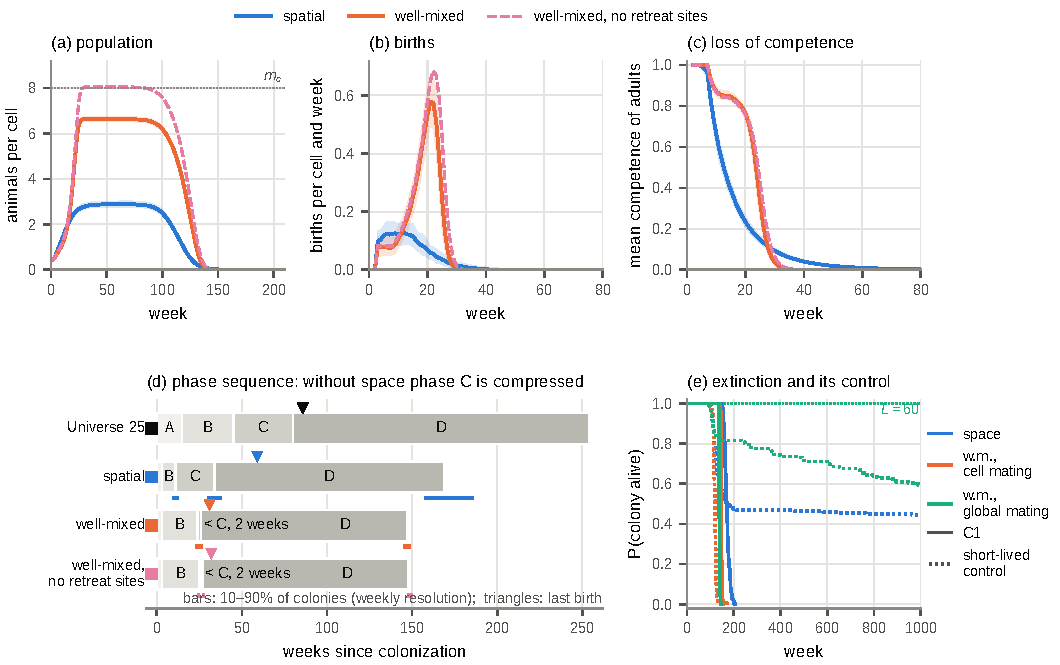
\includegraphics[width=0.92\textwidth]{fig_em_wellmixed.pdf}
  \caption{Extinction with and without space, and its control. Spatial \Cone\ (blue, $n=200$) and well-mixed \Cone,
  in which every animal is relocated at random every week and mates in its cell (orange, $n=200$; retreat sites act
  only as a capacity; pink dashed, without retreat sites, $n=200$); $L=30$, 400 initial animals. (a)~Animals per
  cell; dotted line: the tolerated crowding $m_c$. (b)~Births per cell and week. (c)~Mean reproductive competence of
  the adults. Medians with 10--90\% bands. (d)~Phase sequence of Universe~25 and of each model, dated as in
  Fig.~\ref{fig:trajectory} (medians; bars below: 10--90\% of the colonies at weekly resolution; triangles: last
  birth). With mating in the cell phase~C lasts two weeks. (e)~Kaplan--Meier survival to week $1\,000$ of \Cone\
  (solid) and of the short-lived control (dotted) in space, well mixed with mating in the cell, and well mixed with
  global mating ($L=30$; the control with global mating also at $L=60$, where no colony dies out). Global mating
  appears only in panel~(e). Maps of one colony at its peak and in its decline: SM, Fig.~\ref{SM-fig:snapshots};
  full sequences: Supplementary Videos S1--S3.}
  \label{fig:wellmixed}
\end{figure}

\subsection{Which rule produces which pattern}
\label{sec:res-patterns}

The pattern matrix filters structures through the collapse envelope (Fig.~\ref{fig:patterns}). The envelope passes
in every column with crowding damage and long-lived adults that do not recover fast, except that adult deterioration
before the peak is only partial in the well-mixed core (0.78 of runs with mating in the cell and 0.18 with global
mating): with global mating the core reproduces the end of natality and the extinction, but not
the deterioration of adults before the peak. The envelope fails in the two reversible structures, the
reversible-suppression null and the short-lived control. Without crowding damage the colony explodes (every run
reaches the numerical cap of $15\,000$ animals at weeks 26--29, median 27). The spatial patterns, a peak far below capacity with empty nest sites and
aggregation with free space, pass in every spatial column with crowding damage and in no well-mixed one. All
essential patterns jointly hold in 0.995 [0.97, 1.00] of the runs of \Cone\ (199 of 200) and in none of the other
columns. The senescent nature of the decline holds by construction (there is no social mortality), but its duration
criterion passes in 0.62 of the \Cone\ runs; the persistence of the withdrawn class follows from the capacity of the
retreat sites, which equals the isolation threshold; the failure of transplanted adults follows from R1; and in the
well-mixed columns the coexistence of crowded and withdrawn non-breeders is arithmetic, not behaviour
(Fig.~\ref{fig:patterns}).

The ablations name the rule behind each pattern (SM, Fig.~\ref{SM-fig:ablations}). Without the sensitive window (R1,
adults recovering socially) the envelope is lost (extinction in 0.23 of the runs); without social learning (R2) only
the failure of the late cohorts; without retreat sites (R7) only the persistence of the withdrawn class; without crowd
aversion only the timing clause of the end of natality (0.82) and the duration of the decline. The core model keeps
the envelope in space and loses the cohort failure, the coexistence of classes and their persistence. Over two Latin
hypercubes of 15 factors, 353 of 400 parameter points (0.88, 95\% interval 0.85--0.91) reproduce the collapse
envelope, 168 add the failure of the late cohorts, and 9 reproduce every essential pattern (0.022). The collapse is
generic once adults do not recover; what is rare is its conjunction with the spatial and class patterns. Maternal
transmission is not needed ($w=0$ with faster learning gives 1.00), and at fixed seeding density the joint outcome
rises from 0.82 at $L=15$ to 1.00 at $L\ge45$ (SM, Fig.~\ref{SM-fig:robustness}).

Of the seven confirmatory predictions fixed before the production runs, three fail with each evaluator (SM,
Section~\ref{SM-supp:Q}). Q2, that each rule is necessary, fails because without crowd aversion the joint outcome
stays at 0.79 [0.71, 0.86] (0.90 with the preregistered evaluator) against the predicted $\le0.5$; Q5, a band of
coexisting crowded and withdrawn non-breeders centred at the preferred occupancy, is refuted in the opposite
direction; and Q6, that the window weighs less than the learning rate, fails with the primary evaluator and holds
with the preregistered one. Q1, the failure of transplanted late animals, holds with the primary evaluator but not
with the preregistered one, which takes the transplants at $1.75$ times the week of $\arg\max N$, later in the
plateau: 12 of 60 groups found a colony ($P_T=0.20$ [0.12, 0.32]). Q3, Q4 and Q7 hold with both.

\begin{figure}[!tp]
  \centering
  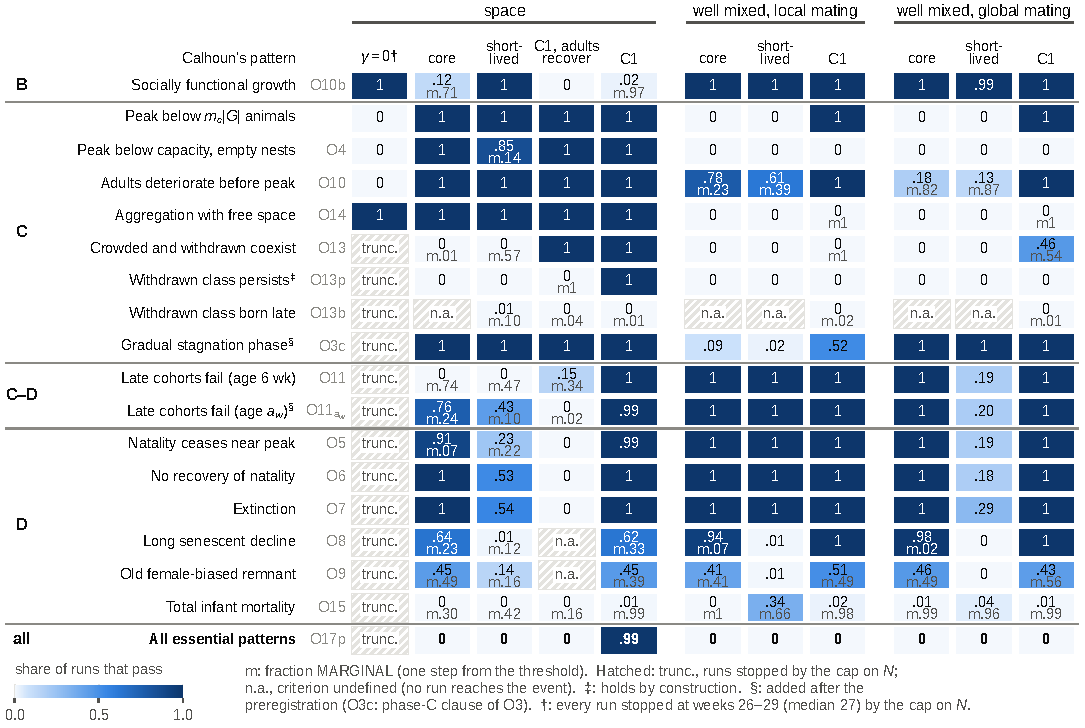
\includegraphics[width=\textwidth]{fig_em_patterns.pdf}
  \caption{Which model structures reproduce Calhoun's patterns. Colour and upper number: fraction of runs that pass
  the operational criterion (primary evaluator, $n=200$ per column, $L=30$, $T=600$; Wilson half-width $\le0.07$);
  lower number (m): fraction MARGINAL, one step from the threshold. Columns: in space, no crowding damage ($\gamma=0$;
  $\dagger$every run stops at weeks 26--29, median 27, when $N$ reaches the numerical cap of $15\,000$, so only
  criteria decided before the cap are shown), the core model (crowding damage, maternal transmission, senescence and attraction,
  without R1, R2, AV and R7), the short-lived control, \Cone\ with adults that recover ($\eadult=0.8$,
  $\lambda=0.9$) and \Cone; well mixed with mating in the cell, and with global mating, for the core model, the
  control and \Cone. Each column comes from one ensemble and seed set (SM, Table~\ref{SM-tab:res-ensembles}). The
  first row is empirical (peak below $m_c|G|$). In the well-mixed columns the
  coexistence of crowded and withdrawn non-breeders is fixed by the capacity of the retreat sites, and the joint
  outcome is 0 by construction (a withdrawn class cannot persist under random relocation). $\ddagger$: holds by
  construction. $\S$: added after the preregistration (the phase-C clause of O3, $t_D-t_{BC}\ge0.1\,t_D$; O11 at
  age $a_w$).}
  \label{fig:patterns}
\end{figure}

\subsection{Behavioural patterns}
\label{sec:res-behaviour}

The individual-level patterns of Calhoun's report appear in the model, each with its ingredient
(Fig.~\ref{fig:behaviour}). In space, crowded and withdrawn non-breeders coexist and the withdrawn class persists: at
week 60, 18\% of the adults are crowded non-breeders, 28\% withdrawn and 17\% persistently withdrawn; well mixed,
isolation is brief and random (57\%, 9\% and 0.2\%). Maternal care fails with the competence of the mothers: the
share of pups that survive birth falls through the growth phase in both variants. The late-born cohorts never breed:
35\% of the females of the first spatial cohort ever conceive, 11\% of those born in week 13 and 6\% of those born in
week 20 (in a two-cell universe run in parallel with Universe~25, 18\% of 148 females born in the last 50 days of
phase~C had ever conceived by a median age of 334 days; \citealp[p.~85]{Calhoun1973}). The transplants of
\citet{Marsden1972}, whose animals bred very poorly rather than not at all, are reproduced qualitatively: groups
taken in the growth phase found a colony in 52 of 60 trials, and those taken in the death phase in none, alone or
with healthy partners (0/60 and 0/120), by the irreversibility built into R1 (Section~\ref{sec:res-recovery}).

\begin{figure}[!tp]
  \centering
  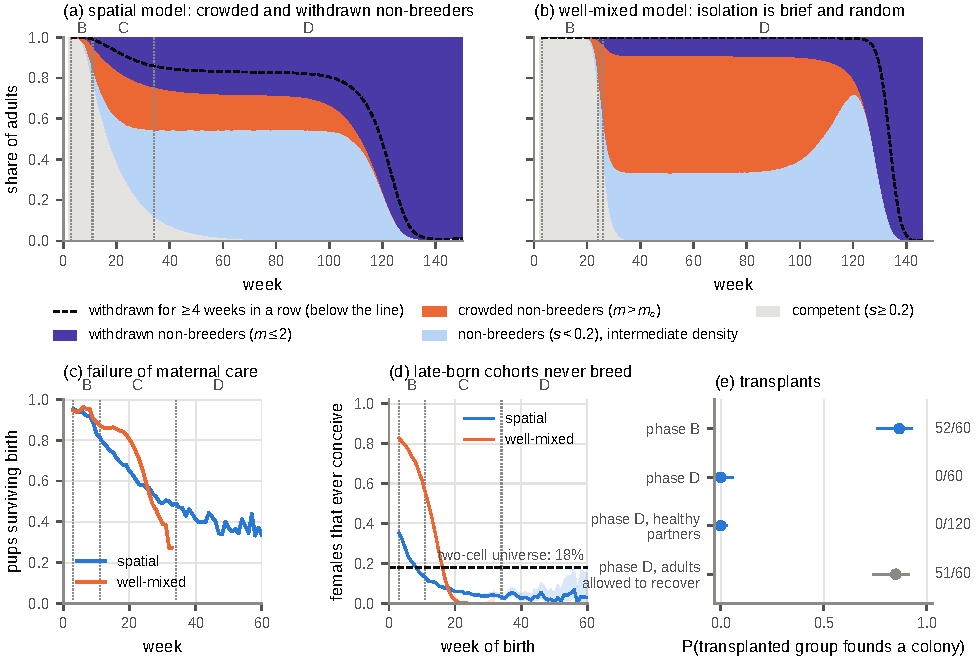
\includegraphics[width=0.9\textwidth]{fig_em_behaviour.pdf}
  \caption{Behavioural patterns. (a,~b)~Composition of the adults (mean over living colonies) in the spatial and the
  well-mixed \Cone: competent ($s\ge0.2$), and non-breeders ($s<0.2$) that are crowded ($m>m_c$), withdrawn (at most
  two animals in the cell) or at intermediate density; below the dashed line, adults withdrawn for at least four
  consecutive weeks. (c)~Share of pups that survive birth, which falls with the competence of the mother (births per
  conception divided by the mean litter size). (d)~Share of the females born in each week that ever conceive, with
  95\% Wilson bands (well mixed: 83\%, 43\% and 2\% for the cohorts born in weeks 3, 13 and 20); dashed line: 18\% of
  the late phase-C females of Calhoun's two-cell universe had ever conceived, a comparison of order (different colony
  and definition). (e)~Transplants (60 groups of four males and four females per arm, 95\% Wilson intervals): a group
  founds a colony when it reaches 80 animals within 150 weeks in an empty enclosure; phase-D animals are taken at
  $1.75\,t'_{\rm pk}$ (primary evaluator). Phase-D animals moved to an
  enclosure where adults may recover (no R1 and R2, individual recovery at rate 0.1) found a colony in 51 of 60
  trials. Dotted lines: phase boundaries of the spatial model (Fig.~\ref{fig:trajectory}).}
  \label{fig:behaviour}
\end{figure}

\subsection{The mechanism}
\label{sec:res-mechanism}

The collapse has the same logic in both structures, a non-breeding state that crowding induces and that adults
cannot leave, but the step that drives it differs. In space, aggregation crowds the adults during growth: the
crowding experienced by juveniles, $\gamma\,\mathrm{E}(m-m_c)_+$, exceeds the maximal gain $r$ only during the growth
phase, when the adults lose their competence within weeks; with $\eadult=0$ they never regain it, and the cohorts
that follow have neither the uncrowded window nor competent neighbours. In the well-mixed limit, the long-lived
non-breeders form a standing stock that keeps the mean crowding above a threshold $\nu^*=6.92$, at which the
expected damage to a juvenile equals $r$; in the kinetic equation, the limit of the well-mixed model at fixed
density, the first cohorts fail through damage inside the window before demonstrators become scarce (SM,
Section~\ref{SM-supp:recovery}). A second threshold, the proportion $\theta^*=(1-w)/(ra_w)=2/3$ of neighbours with
$s>0$, a threshold for the transmission of competence between generations, is only a precursor: in the
simulations the mean proportion around juveniles crosses it before natality falls below 5\% of its maximum, by a
median of 15 weeks in space and 3 well mixed, also in colonies that later persist. Which of these statements are
definitions, analytical arguments, conjectures or simulation results is listed in SM Section~\ref{SM-supp:recovery}. Once the
cohorts mature incompetent, natality stops and the closed colony dies out after the residual life span of the last
cohort, 111 weeks after the last birth in space (median) and about 117 well mixed. In the well-mixed limit two
independent conditions make the non-breeding state absorbing: no adult recovery ($\eadult=0$) or purely social
learning ($\lambda=1$), since an adult whose gain is social cannot recover among non-breeders. Nor is the collapse a
mate-finding Allee effect \citep{Gascoigne2009}: well mixed, \Cone\ collapses with mating in the cell, in the
$3\times3$ block or over the whole arena (50 of 50 colonies under each at $L=15$--60; 95\% interval $[0.93,1]$),
whereas the short-lived control persists with global mating for $L\ge45$ (SM, Table~\ref{SM-tab:sm-mate}).
